\appendix

\chapter{Space Charge Geometry Factors}

\section{Fields of Round Beams}

% \subsection{Longitudinal Fields in a Conducting Cylinder}

% Consider a uniform long cylindrical beam
% \begin{figure}
%     \centering
%     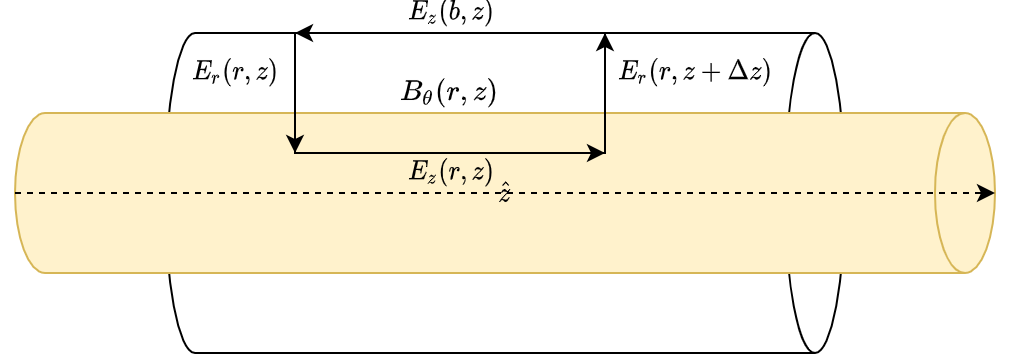
\includegraphics{figs/amperian_surface.drawio.png}
%     \caption{Field Schematic of Coasting Beam}
% \end{figure}

% From ampere's law:

% $$\nabla \times \vec{E} = -\frac{\partial B}{\partial t} \to \oint \vec{E}\cdot d\vec{l} = -\frac{\partial}{\partial t}\iint_S\vec{B}\cdot d\vec{A}$$

% When defining the following integration path/surface through a round charge distribution:

% $$\begin{aligned}
%         \oint \vec{E}\cdot d\vec{l} = E_z(r,z)\Delta z + \int_r^bE_r(r', z+\Delta z)dr'-E_z(b, z)\Delta z -\int_r^bE_r(r', z)dr'
%     \end{aligned}$$

% Because:

% $$\begin{aligned}
%         -\frac{\partial}{\partial t}\iint_S\vec{B}\cdot d\vec{A} = -\Delta z \frac{\partial}{\partial t}\int_r^bB_{\theta}(r', z)
%     \end{aligned}$$

% And that:

% $$E_r(r', z+\Delta z)-E_r(r', z) = \frac{\partial E_r(r', z)}{\partial z}\Delta z$$

% From $dz = -vdt$ we can make the following substitutions:

% $$\begin{aligned}
%         E_z(r,z)-E_z(b,z) & = -\int_r^b\left[\frac{\partial E_r(r', z)}{\partial z}+\frac{\partial B_{\theta}(r', z)}{\partial t}\right]dr' \\
%                           & =-\frac{\partial}{\partial z}\int_r^b[E_r(r',z)-vB_{\theta}(r',z)]dr'                                           \\
%                           & =-\frac{\partial}{\partial z}\int_r^b[E_r(r',z)-\beta^2E_r(r',z)]dr'
%     \end{aligned}$$

% Therefore:

% $$E_z(r,z) = E_z(b,z)-(1-\beta^2)\frac{\partial}{\partial z}\int_r^bE_r(r',z)dr'$$

% For a conducting pipe, $E_z(b,z)=0$ and so the longitudinal self fields are given by:

% $$E_z(r, z) = -\frac{1}{\gamma^2}\frac{\partial}{\partial z}\int_r^bE_r(r', z)dr'$$

% \subsection{Radial Fields in Cylindrical Bunches}

% Considering a cylindrical bunch defined by it's linear charge density $\lambda(z)$, a gaussian element of length $\Delta z$ located at $z$ is defined by:

% $$Q = \lambda(z) \Delta z$$

% \begin{figure}
%     \centering
%     \includegraphics{./figs/gaussian_cylindrical_bunch.drawio.png}
%     \caption{Integration Surfaces to Compute Radial Fields in Cylindrical Beam}
% \end{figure}

% We can define \textit{form factor} $f(r)$, the proportion of charge enclosed in a cylindrical area of radius $r$ given by the radial charge density $\rho(r)$:

% $$f(r) =  \frac{\int_0^r \rho(r') r' dr'}{\int_0^\infty \rho(r') r' dr'} = \frac{Q_{enc}}{Q}$$

% Therefore:

% $$Q_{enc} = f(r) Q = f(r)\lambda(z) \Delta z$$

% From an gaussian cylinder of length $\Delta z$ and radius $r$, we deduce from:

% $$\nabla \cdot \vec{E} = \frac{\rho}{\epsilon_0} \rightarrow \int_S \vec{E}\cdot d\vec{A} = \frac{Q_{enc}}{\epsilon_0}$$

% Such that:

% $$\vec{E_r}(r) \cdot 2\pi r \Delta z = \frac{f(r) \lambda(z)\Delta z}{\epsilon_0}$$

The longitudinal self fields for a round beam in a conductive pipe of radius \textbf{b} is given by
$$E_z(r, z) = -\frac{1}{\gamma^2}\frac{\partial}{\partial z}\int_r^bE_r(r', z)dr'.$$ such that the radial fields can be defined by $$E_r(r, z) = \frac{\lambda(z)}{2\pi\epsilon_0}\frac{f(r)}{r}$$ where $\lambda(z)$ describes the linear charge density \cite{ferrario_space_2014}. Accordingly the longitudinal fields can be defined by
\begin{equation}
    E_z = -\frac{\bar{g}}{2\pi\epsilon_0\gamma^2}\frac{\partial \lambda}{\partial z}
    \label{eq:longitudinal_self_fields}.
\end{equation} where the \textit{geometry factor} \cite{zotter_impedances_1998} $\bar{g}$ is given by
$$\bar{g} = \int_r^b\frac{f(r')}{r'}dr'$$ and the form factor $f(r)$ is defined by $$f(r) =  \frac{1}{Q}\int_0^r \rho(r') r' dr',$$  where $\rho$ is the radial charge density.

\section{Geometry Factors}

\subsection{Uniform Distribution}

A uniform charge distribution in a cylindrical beam is defined by constant surface charge density 
$$\rho(r) = \sigma = \frac{Q}{\pi a^2}.$$ 
Our form factor is therefore given by
$$f(r) = \begin{cases}
        \frac{r^2}{a^2} & r < a \\
        1               & r > a
\end{cases}.$$
Therefore our radial fields are defined by
$$E_r(r,z) = \begin{cases}
    \frac{\lambda(z)}{2\pi\epsilon_0}\frac{r}{a^2} & r < a \\
    \frac{\lambda(z)}{2\pi\epsilon_0}\frac{1}{r}   & r > a
\end{cases},$$
and the geometry factors is given by
$$\begin{aligned}\bar{g}(r<a) &= \int_r^a\frac{r'}{a^2}dr'+\int_a^b\frac{1}{r'}dr' \\     \bar{g}(r>a) &= \int_r^b\frac{1}{r'}dr'\end{aligned}$$
Therefore:
\begin{equation}
    \bar{g}(r) = \begin{cases}
        \ln(\frac{b}{a})+\frac{1}{2}-\frac{1}{2}\frac{r^2}{a^2} & r < a \\
        \ln(\frac{b}{r})                                        & r > a
    \end{cases}
    \label{eq:g_uniform}.
\end{equation}

\subsection{Parabolic Distribution}

A parabolic charge distribution of radius $a$ yields the following charge profile:
$$\rho(r) = \frac{2Q}{\pi a^2}\left(1-\frac{r^2}{a^2}\right).$$
where
$$Q = \int_0^a \rho(r) r dr.$$
The form factor is given by
$$\begin{aligned}f(r<a) = \frac{2\pi}{Q}\int_0^r\rho(r')r'dr' \\ f(r > a) = 1\end{aligned}$$
The form factor is therefore given by
$$f(r) = \begin{cases} 2\frac{r^2}{a^2}-\frac{r^4}{a^4} & r < a\\
1 & r > a
\end{cases}$$
Therefore the geometric factor is given by
$$\begin{aligned}
\bar{g}(r<a) & = \int_r^a \frac{1}{r'}\left(2\frac{r'^2}{a^2}-\frac{r'^4}{a^4}\right)dr'+ \int_a^b\frac{1}{r'}dr' \\
\bar{g}(r>a) &= \int_r^b\frac{1}{r'}dr'
\end{aligned}$$
Therefore:
\begin{equation}
    \bar{g}(r) = \begin{cases}
        \ln\left(\frac{b}{a}\right)+\frac{a^2-r^2}{a^2}-\frac{a^4-r^4}{4a^4} & r < a \\
        \ln(\frac{b}{a})                                                     & r > a\end{cases}
    \label{eq:g_parabolic}.
\end{equation}

\subsection{Gaussian Distribution}

Given a radial charge distribution for a gaussian beam is defined by
$$\rho(r) = \frac{Q}{\sigma_r^2(\sqrt{2\pi})^2}\exp\left(-\frac{r^2}{2\sigma_r^2}\right)$$
the form factor is generalized by
$$f(r) = 1-\exp\left(-\frac{r^2}{2\sigma_r^2}\right)$$
Therefore
$$\begin{aligned}
        \bar{g}(r) & = \int_r^b\frac{1}{r'}\left(1-\exp\left(-\frac{r'^2}{2\sigma_r^2}\right)\right)dr'                                            \\
             & =\int_r^b\frac{dr'}{r'} -\int_r^b\frac{1}{r'}\exp\left(-\frac{r^2}{2\sigma_r^2}\right)dr'                                     \\
             & = \ln(r')\Big|_r^b -\frac{1}{2}\text{Ei}\left(-\frac{r'^2}{2\sigma_r^2}\right)\Big|_r^b                                       \\
             & = \ln\left(\frac{b}{r}\right)-\frac{1}{2}\left(\text{Ei}(-\frac{b^2}{2\sigma_r^2})-\text{Ei}(-\frac{r^2}{2\sigma_r^2})\right)
    \end{aligned}$$
Or more concisely
\begin{equation}
    \bar{g}(r) = \ln\frac{b}{r} + \frac{1}{2}\left(\rm{Ei}(-\frac{1}{2}\frac{r^2}{\sigma_r^2})-\rm{Ei}(-\frac{1}{2}\frac{b^2}{\sigma_r^2})\right)
    \label{eq:g_gaussian}.
\end{equation}
where the exponential integral $\text{Ei}$ is defined by \cite{abramowitz_handbook_2013} % p228
$$\text{Ei}(x) = \int_{-\infty}^x \frac{e^t}{t}dt.$$
The maximum value occurs at
$$\bar{g}(r=0) = \frac{1}{2}\left(\ln\left(\frac{b^2}{2\sigma_r^2}\right)+\Gamma(0, \frac{b^2}{2\sigma_r^2}+\gamma\right)$$
where $$\Gamma(a, x) = \frac{1}{\Gamma(a)}\int_0^xt^{a-1}e^{-t}dt$$
and the Euler–Mascheroni constant is given by
$$\gamma = \lim_{n\to\infty}\left(-\ln n +\sum_{k=1}^n\frac{1}{k}\right) \approx 0.57721.$$
The geometry factor can be approximated by that for a truncated gaussian can be given by \cite{ng_space-charge_2004,ng_physics_2006}
$$\bar{g}(r<m\sigma_r) = \frac{\gamma+2\ln\frac{b}{\sigma_r\sqrt{2}}+E_1(\frac{m^2}{2})}{1-\exp(-m^2/2)}.$$

\chapter{Möller–Trumbore Algorithm}

This easily parallelized algorithm can efficiently detect and compute the intersections of a ray $q=(q_0, q_1)$ through a face $p=(p_0, p_1, p_2)$. The interaction between a ray and a face can be characterized as \textbf{intersecting} and \textbf{non-intersecting}
\begin{figure}
    \centering
    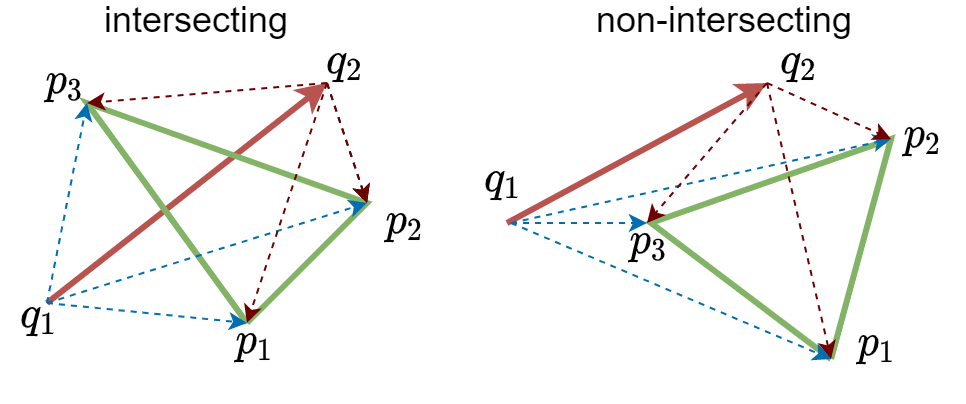
\includegraphics{figs/moller_trumbore.drawio.png}
\end{figure}

The signed volumes of possible tetrahedron combinations is given by
$$\begin{aligned}
    s_1 = \text{sign}(V(q_1, p_1, p_2, p_3))\\
    s_2 = \text{sign}(V(q_2, p_1, p_2, p_3))\\
    s_3 = \text{sign}(V(q_1, q_2, p_1, p_2))\\
    s_4 = \text{sign}(V(q_1, q_2, p_2, p_3))\\
    s_5 = \text{sign}(V(q_1, q_2, p_3, p_1))\\
\end{aligned}$$
where the volume of a tetrahedron is defined by
$$V(a, b, c, d) = \frac{1}{6} \left((d-a) \cdot ((b-a) \times (c-a))\right).$$
An intersection exists if 
\begin{equation}
    s_1 \neq s_2 \quad \& \quad s_3 = s_4 \quad \& \quad s_4 = s_5.
    \label{eq:moller}
\end{equation}
The intersection point $q_0$ is then given by
$$q_0 = q_1 + t (q_2-q_1) \qquad t = \frac{(p_1-q_1) \cdot n}{(q_2-q_1) \cdot n} \qquad n = (p_2-p_1) \times (p_3-p_1).$$

% \chapter{Expressions for Phase Advance in the PS}

% Suppose we can approximate our optics $\beta_m$ about a ring's polar position $s = R\theta$ by complex Fourier coefficients $\beta_k$:

% $$\beta_m = \sum_{k=0}^{n-1}\beta_k\exp(2\pi i \frac{m k}{n}) \to \beta(\theta) \approx \beta_0 + \sum_{k=1}^{n-1}|\beta_k|\cos(k\theta+\varphi_k)$$

% where:

% $$s_m = \frac{m}{n}\mathcal{C} \qquad s = R\theta$$

% \section{First Order Approximation}

% Approximating such that:

% $$\beta(s) \approx |\beta_0| \qquad D(s) = |D_0|$$

% Our phase advance is simply:

% $$\mu(s) = \frac{s}{|\beta_0|}$$

% Our trajectories are therefore:

% $$\begin{aligned}
%         x(s) & \approx \sqrt{|\beta_{0,x}|\epsilon_x}\cos(\frac{s}{|\beta_{0,x}|}+\mu_{0,x})+|D_{0,x}| \delta \\
%         y(s) & \approx \sqrt{|\beta_{0,y}|\epsilon_y}\cos(\frac{s}{|\beta_{0,y}|}+\mu_{0,y})
%     \end{aligned}$$

% We may notice for the \textbf{PS} that $\beta_{0,x} \approx \beta_{0,y}$

% Our matched transverse gaussian bunch may be generated using the covariance matrix $\Sigma = \epsilon \Omega$ where:

% $$\Omega = \begin{pmatrix}\beta & -\alpha\\-\alpha & \gamma\end{pmatrix} \qquad \alpha = -\frac{\beta'}{2} \qquad \gamma = \frac{1+\alpha^2}{\beta}$$

% \section{Second Order Approximation}

% Consider we take the first coefficient $k=0$ and the next most significant mode $k$ to describe our oscillations such that:

% $$\begin{aligned}
%         \beta(s=R\theta) & \approx \beta_0 + |\beta_k|\cos(k\theta+\varphi_k) \\
%         D(s=R\theta)     & \approx D_0 + |D_k|\cos(k\theta + \varphi_k)
%     \end{aligned}$$

% For the \textbf{PS}, we observe a symmetry such that:

% $$\beta_x(\theta) \approx \beta_y(\theta+\frac{\pi}{k})$$

% And so our phase advance can be computed analytically, allowing us to apply a "kick" to the phase-advance tracked in longitudinal tracking codes:

% $$\mu(s) =\int_0^{s}\frac{ds'}{\beta(s)} \to \mu(\theta) = \int_{\theta_0}^{\theta}\frac{Rd\theta}{\beta_0+|\beta_k|\cos(k\theta+\varphi_k)}
%     =$$

% $$\boxed{\mu(\theta) \approx -\frac{2R}{k\sqrt{|\beta_k|^2-\beta_0^2}}\tanh^{-1}\left(\frac{(|\beta_k|-\beta_0)\tan(\frac{1}{2}(k\theta+\varphi_k))}{\sqrt{|\beta_k|^2-\beta_0^2}}\right)}$$